\chapter{Tree Compression Scheme} \label{chp:project_overview}
As introduced in the first chapter, the primary goal of this thesis is to develop a novel tree compression scheme that effectively leverages repetitive structures within the input trie. The proposed algorithm is designed to identify and compactly represent these recurring patterns, thereby improving compression performance, particularly for highly repetitive tries. This chapter provides an overview of the proposed compression scheme.

\section{Compression Scheme Pipeline}
The overall pipeline of our proposed method is outlined in Algorithm~\ref{alg:pipeline}. It takes an input trie $T$ and a width parameter $p$ and produces a compressed, $p$--sortable automaton.
\begin{algorithm}[H]
\caption{$\textsc{CompressTrie}(T,p)$}
\label{alg:pipeline}
\begin{algorithmic}[1]
\Require Input trie $T$, width integer parameter $p$
\Ensure A compressed, $p$--sortable automaton $\mathcal{A}$
    \State $V_{sorted} = \textsc{PathSort}(T)$ 
    \State $N[1,\dots,|Q|] = \text{RevuzMinimization}(T)$
    \State $G_{bipartite} = \text{ConstructMWPBMInstance}(V_{sorted}, N, p)$
    \State $M = \text{SolveMWPBM}(G_{bipartite})$ 
    \State $C[1,\dots,p] = \text{ExtractChainsFromMatching}(M, V_{sorted})$ 
    \State $\mathcal{A} = \text{CollapseChains}(C, N)$ 
    \State \Return $\mathcal{A}$
\end{algorithmic}
\end{algorithm}

The first step of the pipeline (line 2) establishes a total order on the nodes of the trie. This is achieved by sorting the nodes co--lexicographically using the \textbf{Path Sort} algorithm, which we described in \cref{alg:pathSort}. This sorting is fundamental, as it arranges the nodes in the order required for a Wheeler automaton.

Next, the algorithm identifies which nodes are candidates for merging (line 3). This is done by partitioning the nodes into equivalence classes based on the structure of the subtrees rooted at each node. Two nodes are in the same class if and only if their subtrees are isomorphic. This is equivalent to computing the Myhill--Nerode equivalence classes for the finite language accepted by the trie, a process we adapt from Revuz's algorithm for minimizing acyclic DFAs (\cref{alg:minimization-ADFA}).

The core of the algorithm lies in lines 4 and 5, where we solve the \textbf{String Partitioning Problem}. The input to this problem is the string formed by concatenating the Myhill--Nerode classes of the sorted nodes. As detailed in \cref{sec:reduction_to_mwpbm}, we reduce this problem to finding a Minimum Weight Perfect Bipartite Matching (MWPBM). A bipartite graph is constructed where the weight of each edge corresponds to the cost of placing two characters adjacently in a subsequence. By finding a perfect matching with minimum weight using standard algorithms (\cref{sec:mwpbm_solutions}), we can reconstruct a partition of the string into $p$ subsequences that minimizes the total number of runs, thereby maximizing compression.

Finally, the DAG compressed automaton is constructed (line 6). The algorithm iterates through each of the $p$ subsequences and ``collapses'' any consecutive sequence of nodes belonging to the same Myhill--Nerode equivalence class into a single state. This compression, which we describe in \cref{sec:collapsing}, produces the final $p$--sortable automaton, which can then be indexed for efficient querying (\cref{sec:indexing}).

\begin{example}[Compression pipeline] \label{ex:string_example}
    In our running example, we begin with the tree shown in \cref{fig:mn-compressed-tree}. Each node in this tree is labeled with its corresponding Myhill--Nerode equivalence class, as determined in \cref{ex:ADFA_minimization}. By traversing the nodes in co--lexicographic order, we construct a string $S$ where each character represents the Myhill--Nerode equivalence class of a node:
    \[
        S = \text{ABCDDCBDDDD}
    \]
    This string $S$ then becomes the input to the String Partitioning Problem (see \cref{def:string_partitioning_problem}), where the objective is to partition $S$ into $p$ subsequences while minimizing the total number of runs.

    % First figure - Original tree
    \begin{figure}[H]
        \centering
        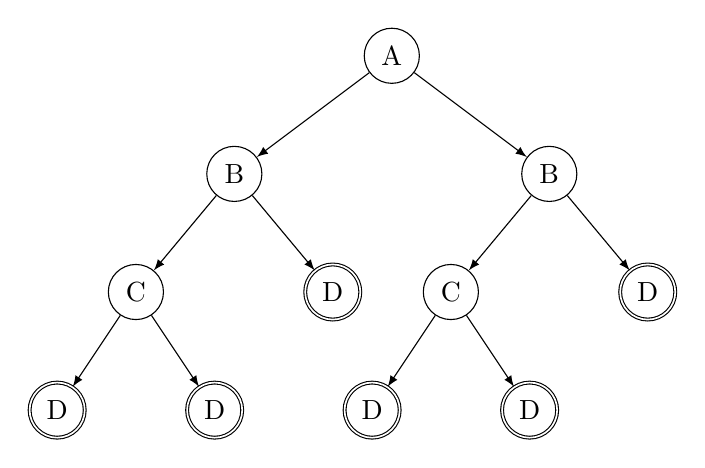
\begin{tikzpicture}[
    level distance=1.5cm,
    sibling distance=3cm,
    state/.style={circle, draw, minimum size=7mm},
    accepting/.style={circle, draw, double, minimum size=7mm},
    edge from parent/.style={draw, -latex},
    level 1/.style={sibling distance=4cm},
    level 2/.style={sibling distance=2.5cm},
    level 3/.style={sibling distance=2cm}
    ]

\node[state] (a) {A}
    child {node[state] (b) {B} 
    child {node[state] (d) {C}
        child {node[accepting] (h) {D}}
        child {node[accepting] (i) {D}}
    }
    child {node[accepting] (e) {D}}
    }
    child {node[state] (c) {B}
    child {node[state] (f) {C}
        child {node[accepting] (l) {D}}
        child {node[accepting] (m) {D}}
    }
    child {node[accepting] (g) {D}}
    };
\end{tikzpicture}
        \caption{Tree ADFA of \cref{fig:example_ADFA}, with each node labeled with its equivalence class.}
        \label{fig:mn-compressed-tree}
    \end{figure}

    Given $p = 2$, one way to partition the string is $C = [\text{ABCDCBD}, \text{DDDD}]$, which is clearly suboptimal as the total number of runs is $runs(C) = 7 + 1 = 8$.
    An optimal solution would be $C' = [\text{ABCCB}, \text{DDDDDD}]$, since $runs(C') = 4 + 1 = 5$ is the minimum number of runs for the partition of $S$ into two chains.
    
\end{example}